\documentclass[letterpaper,twocolumn,10pt]{article}
\usepackage{usenix,epsfig,endnotes}

\usepackage[utf8]{inputenc}
\usepackage[T1]{fontenc}
\usepackage{hyperref}
\usepackage{url}
\usepackage{booktabs}
\usepackage{amsfonts}
\usepackage{microtype}
\usepackage{natbib}
\usepackage{amsmath}
\usepackage{amssymb}
\usepackage{amsthm}
\usepackage{mathtools}
\usepackage{subcaption}
\usepackage{caption}
\usepackage{setspace}
\usepackage{graphicx}
\usepackage[margin=1in]{geometry}
\usepackage{color}
\usepackage{graphics, enumitem}
\hypersetup{
  colorlinks=true,
  linkcolor=blue,
  citecolor=magenta,
  filecolor=cyan,
  urlcolor=red
}

\setlength\intextsep{0pt}

\newenvironment{denseitemize}{
\begin{itemize}[topsep=2.5pt, partopsep=0pt, leftmargin=1.5em]
  \setlength{\itemsep}{2.5pt}
  \setlength{\parskip}{0pt}
  \setlength{\parsep}{0pt}
}{\end{itemize}}

\newenvironment{denseenum}{
\begin{enumerate}[topsep=2.5pt, partopsep=0pt, leftmargin=1.5em]
  \setlength{\itemsep}{2.5pt}
  \setlength{\parskip}{0pt}
  \setlength{\parsep}{0pt}
}{\end{enumerate}}


\title{CS498 MLsys Project Report:\\Reproducing and Extending Learning to Draft:\\Adaptive Speculative Decoding with Reinforcement Learning}

\author{
\hspace{1.0cm} Zifan Ying \hspace{2.5cm} Shaoshao Xiong \\
\hspace{0.4cm} zifany4@illinois.edu \hspace{0.8cm} sx24@illinois.edu
}

\newcommand{\mbb}[1]{\mathbb{#1}}
\newcommand{\mbbC}{\mbb{C}}
\newcommand{\mbbE}{\mbb{E}}
\newcommand{\mbbQ}{\mbb{Q}}
\newcommand{\mbbR}{\mbb{R}}
\newcommand{\mbbZ}{\mbb{Z}}
\newcommand{\mbbI}{\mbb{I}}

\newcommand{\mc}[1]{\mathcal{#1}}
\newcommand{\mcA}{\mc{A}}
\newcommand{\mcD}{\mc{D}}
\newcommand{\mcF}{\mc{F}}
\newcommand{\mcM}{\mc{M}}
\newcommand{\mcN}{\mc{N}}
\newcommand{\mcP}{\mc{P}}
\newcommand{\mcS}{\mc{S}}
\newcommand{\mcX}{\mc{X}}
\newcommand{\mcY}{\mc{Y}}
\newcommand{\mcZ}{\mc{Z}}

\newcommand{\mbf}[1]{\mathbf{#1}}
\newcommand{\mbA}{\mbf{A}}
\newcommand{\mbB}{\mbf{B}}
\newcommand{\mbD}{\mbf{D}}
\newcommand{\mbI}{\mbf{I}}
\newcommand{\mbK}{\mbf{K}}
\newcommand{\mbM}{\mbf{M}}
\newcommand{\mbQ}{\mbf{Q}}
\newcommand{\mbR}{\mbf{R}}
\newcommand{\mbS}{\mbf{S}}
\newcommand{\mbU}{\mbf{U}}
\newcommand{\mbV}{\mbf{V}}
\newcommand{\mbW}{\mbf{W}}
\newcommand{\mbX}{\mbf{X}}
\newcommand{\mbY}{\mbf{Y}}
\newcommand{\mbZ}{\mbf{Z}}
\newcommand{\mbc}{\mbf{c}}
\newcommand{\mbe}{\mbf{e}}
\newcommand{\mbx}{\mbf{x}}
\newcommand{\mby}{\mbf{y}}
\newcommand{\mbGamma}{\mbf{\Gamma}}
\newcommand{\mbSig}{\mbf{\Sigma}}
\newcommand{\mbPhi}{\mbf{\Phi}}
\newcommand{\mbPsi}{\mbf{\Psi}}
\newcommand{\mbalpha}{\bm{\alpha}}
\newcommand{\mbbeta}{\bm{\beta}}
\newcommand{\mbphi}{\bm{\phi}}
\newcommand{\mbpsi}{\bm{\psi}}
\newcommand{\mbxi}{\bm{\xi}}
\newcommand{\mbone}{\bm{1}}


\newcommand{\fitp}[1]{ \left( #1 \right) }
\newcommand{\fitcb}[1]{ \left \{ #1 \right \} }
\newcommand{\fitsb}[1]{ \left[ #1 \right] }
\newcommand{\fitab}[1]{ \left \langle #1 \right \rangle }
\newcommand{\norm}[1]{\left\lVert#1\right\rVert}

\newcommand{\tn}[1]{\textnormal{#1}}
\newcommand{\tnb}[1]{\textnormal{\textbf{#1}}}

\newcommand{\argmax}[1]{\tn{arg} \max_{#1}}
\newcommand{\argmin}[1]{\tn{arg} \min_{#1}}
\newcommand{\argsup}[1]{\tn{arg} \sup_{#1}}
\newcommand{\arginf}[1]{\tn{arg} \inf_{#1}}

\newcommand{\ddx}[1]{\frac{\partial}{\partial #1}}
\newcommand{\ddxdy}[2]{\frac{\partial^2}{\partial #1 \partial #2}}
\newcommand{\ddxdydz}[3]{\frac{\partial^3}{\partial #1 \partial #2 \partial #3}}

\newcommand{\expec}[2]{ \mbbE_{#1} \fitsb{#2} }

\newcommand{\betapdf}[3]{\frac{\Gamma \fitp{#1} \Gamma \fitp{#2}}{\Gamma \fitp{#1 + #2}} #3^{#1 - 1}(1 - #3)^{#2 - 1}}

\begin{document}

\maketitle

\section{Introduction}

Large language model (LLM) inference is bottlenecked by autoregressive decoding, in which tokens are generated one at a time, preventing effective hardware utilization. Speculative decoding~\cite{leviathan2023fast} addresses this by letting a smaller \emph{draft} model propose candidate token sequences that the target model then verifies in parallel. The key trade-off is that draft quality and verification cost are interdependent: deeper drafts yield more accepted tokens per step but require more verification compute, while shallow drafts are cheap to verify but frequently rejected.

Learning to Draft (LTD)~\cite{ltd2025} is a recent ICLR 2026 paper that frames this trade-off as a reinforcement learning (RL) problem. Built on top of EAGLE-3~\cite{eagle3}, LTD trains two separate PPO policies that at each decoding step decide (1) \emph{how many} draft tokens to propose (the ``size'' controller) and (2) \emph{how deep} to grow the draft tree before stopping (the ``depth'' controller). By optimizing directly for throughput, LTD achieves up to 36.4\% improvement over static EAGLE-3 in greedy decoding settings.

This project aims to reproduce LTD's results, extend them to additional models and datasets not evaluated in the paper, and analyze when adaptive control provides the most benefit. This report summarizes our reproduction results and recent extensions on quantization transfer, hardware transfer, and multi-GPU deployment.

\section{Background}

\paragraph{Speculative Decoding.}
Speculative decoding accelerates autoregressive generation by using a lightweight draft model to propose candidate tokens and a larger target model to verify them in parallel~\cite{leviathan2023fast,chen2023accelerating}. In the lossless setting, this procedure preserves the output distribution of the target model while reducing decoding latency. Beyond the original chain-based formulation, later work introduced tree-structured drafting and parallel verification, which substantially improved practical speedup~\cite{specinfer,eagle2,medusa}.

\paragraph{EAGLE-3.}
EAGLE-3 is a strong tree-based speculative decoding framework built on the EAGLE line of work~\cite{eagle3,eagle2}. Instead of verifying a single drafted chain, it constructs a draft tree and lets the target model verify multiple candidate paths in one forward pass. Its performance depends on a trade-off between draft cost and verification cost: deeper trees and larger verification sets may increase the number of accepted tokens, but they also increase latency.

\paragraph{Learning to Draft.}
Learning to Draft (LTD) formulates speculative decoding as a reinforcement learning problem and replaces EAGLE-3's static control strategy with two adaptive policies~\cite{ltd2025}. Importantly, the two policies control \emph{draft depth} and \emph{verification size}, respectively. The depth policy decides whether to continue expanding the draft tree after each draft-model forward pass, while the size policy selects how many candidate tokens from the generated draft tree should be sent to the target model for verification. Both policies are optimized with PPO using throughput as the reward, directly balancing acceptance length against wall-clock latency~\cite{schulman2017ppo,sb3}.

The core claim of LTD is that speculative decoding should optimize throughput rather than acceptance length alone. The paper reports speedup ratios ranging from 2.24$\times$ to 4.32$\times$, and up to 36.4\% improvement over a strong EAGLE-3 baseline in greedy decoding settings~\cite{ltd2025}. Our project reproduces this idea on five target models and extends the evaluation to a broader set of datasets than those emphasized in the original main results.

\section{Implementation}

\paragraph{RL Training.}
We implement the size and depth controllers as PPO agents using Stable-Baselines3~\cite{sb3}. Training is performed on a single GPU using the EAGLE-3 inference loop as the environment. At each RL timestep, the agent observes a feature vector and takes a discrete action.

The \emph{size policy} uses a 1268-dimensional observation vector comprising the EA layer's candidate confidence scores (1210 floats), current sequence length (29 floats), and a step counter (29 floats). Its action space is the draft token budget. The policy network has hidden layers of size $[1024, 256]$ and is trained for 100\,000 PPO timesteps with learning rate $10^{-3}$, discount $\gamma = 0.9$, entropy coefficient 0.01, and batch size 256.

The \emph{depth policy} uses a 128-dimensional observation vector comprising per-level confidence scores (100 floats), context-length features (14 floats), and a step counter (14 floats). It is trained as a binary stop/continue classifier for 1\,000\,000 timesteps with $\gamma = 0.999$ and a single hidden layer of size 1024.

\paragraph{Models.}
We train and evaluate controllers for five target models spanning different model families and scales:
\begin{denseitemize}
  \item \textbf{Llama-3.1-8B-Instruct} with EAGLE3-LLaMA3.1-Instruct-8B
  \item \textbf{DeepSeek-R1-Distill-Llama-8B} with EAGLE3-DeepSeek-R1-Distill-LLaMA-8B
  \item \textbf{Qwen3-14B} with Qwen3-14B\_eagle3
  \item \textbf{Qwen3-32B} with Qwen3-32B\_eagle3 under 8-bit quantization
  \item \textbf{Vicuna-13B-v1.3} with EAGLE3-Vicuna1.3-13B
\end{denseitemize}
Each model has its own size and depth policy checkpoint trained from scratch.

\paragraph{Datasets.}
We train controllers on the HumanEval coding dataset. For benchmarking, we evaluate on 11 datasets covering diverse task types: \textit{alpaca} (instruction following), \textit{gsm8k} (grade-school math), \textit{humaneval} (code generation), \textit{mt\_bench} (multi-turn dialog), \textit{qa} (question answering), \textit{sum} (summarization), \textit{math} (competition math), \textit{leetcode} (algorithmic coding), \textit{mmlu} (multi-subject knowledge), \textit{bbh} (big-bench hard), and \textit{theoremqa} (theorem proving). This extends the LTD paper, which evaluated on a subset of these tasks.

\section{Evaluation Setup}

We use greedy decoding (temperature 0.0) to match the primary setting emphasized in the LTD paper~\cite{ltd2025}. The initial reproduction experiments run on a single NVIDIA GPU with CUDA and use the same 11-dataset benchmark suite. The new Qwen3-32B reproduction runs on an H100 using 8-bit quantization with 20 samples per dataset, while the quantization-transfer and hardware-transfer sweeps use 50 samples on four representative datasets: HumanEval, Alpaca, GSM8K, and MT-Bench. All runs cap generation at 256 output tokens.

For transfer experiments, we change only the deployment condition while reusing trained policies. Quantization transfer evaluates Qwen3-14B policies trained under bf16, int4, and int8 against all three evaluation precisions. Hardware transfer evaluates bf16 Qwen3-14B policies trained on H100 or A5090 when deployed on an RTX A6000. Finally, the multi-GPU experiment evaluates Qwen3-32B under naive model parallelism with HuggingFace's automatic device map, which shards layers across two GPUs without adding pipeline overlap.

We evaluate on 11 datasets spanning instruction following, reasoning, coding, QA, summarization, and broad knowledge: Alpaca~\cite{taori2023alpaca}, GSM8K~\cite{cobbe2021gsm8k}, HumanEval~\cite{chen2021humaneval}, MT-Bench~\cite{zheng2023mtbench}, Natural Questions-style QA~\cite{kwiatkowski2019natural}, MMLU~\cite{hendrycks2020mmlu}, BBH~\cite{srivastava2023bbh}, and several additional datasets used in our extension experiments.

We report three metrics:
\begin{denseitemize}
  \item \textbf{Throughput} (tokens/second): generated tokens divided by wall-clock time.
  \item \textbf{Speedup}: ratio of method throughput to autoregressive baseline throughput.
  \item \textbf{Avg.\ acceptance length}: mean number of accepted tokens per speculative step.
\end{denseitemize}

We compare three configurations: (1) \emph{Baseline}, standard autoregressive decoding with the target model; (2) \emph{Eagle3}, static EAGLE-3; and (3) \emph{Eagle3+RL}, EAGLE-3 augmented with the LTD-style adaptive size and depth controllers trained in this work.

\section{Results}

\begin{figure}[t]
  \centering
  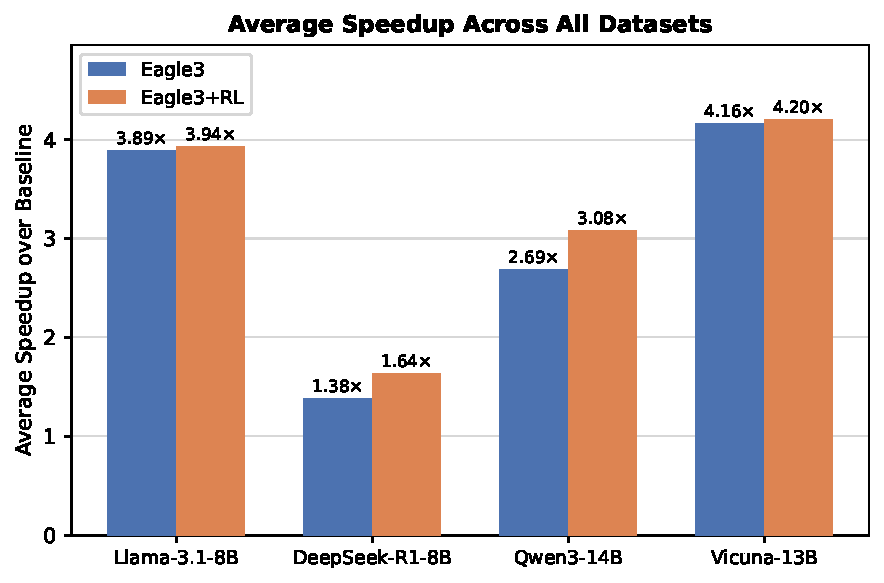
\includegraphics[width=\linewidth]{fig1_avg_speedup.pdf}
  \caption{Average speedup over the autoregressive baseline across all 11 datasets for the initial four-model reproduction. Each pair of bars shows Eagle3 (blue) and Eagle3+RL (orange) for one model. DeepSeek-R1-8B shows the largest \emph{relative} gain; Qwen3-14B shows the largest \emph{absolute} gain.}
  \label{fig:avg_speedup}
\end{figure}

\begin{table}[t]
\centering
\caption{Average speedup over autoregressive baseline across all 11 datasets for the initial four reproduced models. Eagle3+RL uses the LTD-style adaptive controllers trained in this work.}
\label{tab:speedup}
\small
\begin{tabular}{lcc}
\toprule
\textbf{Model} & \textbf{Eagle3} & \textbf{Eagle3+RL} \\
\midrule
Llama-3.1-8B-Instruct        & 3.89$\times$ & \textbf{3.94}$\times$ \\
DeepSeek-R1-Distill-Llama-8B & 1.38$\times$ & \textbf{1.64}$\times$ \\
Qwen3-14B                    & 2.69$\times$ & \textbf{3.08}$\times$ \\
Vicuna-13B-v1.3              & 4.16$\times$ & \textbf{4.20}$\times$ \\
\bottomrule
\end{tabular}
\end{table}

\begin{table}[t]
\centering
\caption{Per-dataset speedup for Qwen3-14B. Eagle3+RL consistently outperforms Eagle3 across all task categories.}
\label{tab:qwen}
\small
\begin{tabular}{lcc}
\toprule
\textbf{Dataset} & \textbf{Eagle3} & \textbf{Eagle3+RL} \\
\midrule
alpaca      & 2.51$\times$ & 2.93$\times$ \\
gsm8k       & 3.05$\times$ & 3.42$\times$ \\
humaneval   & 2.73$\times$ & 3.19$\times$ \\
mt\_bench   & 2.63$\times$ & 3.03$\times$ \\
qa          & 2.30$\times$ & 2.68$\times$ \\
sum         & 2.18$\times$ & 2.55$\times$ \\
math        & 2.99$\times$ & 3.35$\times$ \\
leetcode    & 2.78$\times$ & 3.21$\times$ \\
mmlu        & 2.79$\times$ & 3.18$\times$ \\
bbh         & 2.78$\times$ & 3.17$\times$ \\
theoremqa   & 2.83$\times$ & 3.19$\times$ \\
\bottomrule
\end{tabular}
\end{table}

\paragraph{Overall speedup.}
Table~\ref{tab:speedup} summarizes the average speedup across all 11 datasets for the initial four-model reproduction. Eagle3+RL improves over static Eagle3 for all four models. The gains, however, are highly model-dependent: they are small for Llama-3.1-8B and Vicuna-13B, but much larger for DeepSeek-R1-Distill-Llama-8B and Qwen3-14B. This matches the central LTD hypothesis that adaptive control is most useful when the best speculative-decoding budget varies substantially across contexts~\cite{ltd2025}.

\paragraph{Llama-3.1-8B-Instruct.}
Eagle3 already achieves strong speedups of 3.28$\times$--4.59$\times$ on this model, and the RL controller adds only a modest average gain from 3.89$\times$ to 3.94$\times$. Static acceptance lengths are already high, and in several datasets the RL controller changes acceptance length only marginally. This suggests that the Llama-3.1 draft/verification pair is already close to a saturated operating point under static Eagle3 settings.

\paragraph{DeepSeek-R1-Distill-Llama-8B.}
DeepSeek-R1-Distill-Llama-8B shows the largest \emph{relative} gain from adaptive control: the average speedup increases from 1.38$\times$ to 1.64$\times$, corresponding to roughly 18.8\% relative improvement. Its static acceptance lengths are much lower than those of Llama and Vicuna, indicating that speculative verification is harder on this reasoning-oriented model. In this regime, adaptive control is particularly useful because it can avoid wasting compute on low-value draft expansions.

\paragraph{Qwen3-14B.}
Qwen3-14B shows the largest \emph{absolute} average gain among the reproduced models, improving from 2.69$\times$ to 3.08$\times$ on average. Table~\ref{tab:qwen} shows that the improvement is consistent across all 11 datasets, with gains ranging from about $+$0.37$\times$ to $+$0.46$\times$. This stability is notable because the controllers were trained on HumanEval but still transfer well to dialogue, QA, summarization, and knowledge-heavy benchmarks.

Figure~\ref{fig:qwen_per_dataset} plots the per-dataset speedup gain ($\text{Eagle3+RL} - \text{Eagle3}$) for Qwen3-14B. All 11 bars are positive and the gains are roughly uniform (0.37--0.46$\times$), providing strong evidence that the learned controller generalises well beyond its HumanEval training distribution.

\begin{figure}[t]
  \centering
  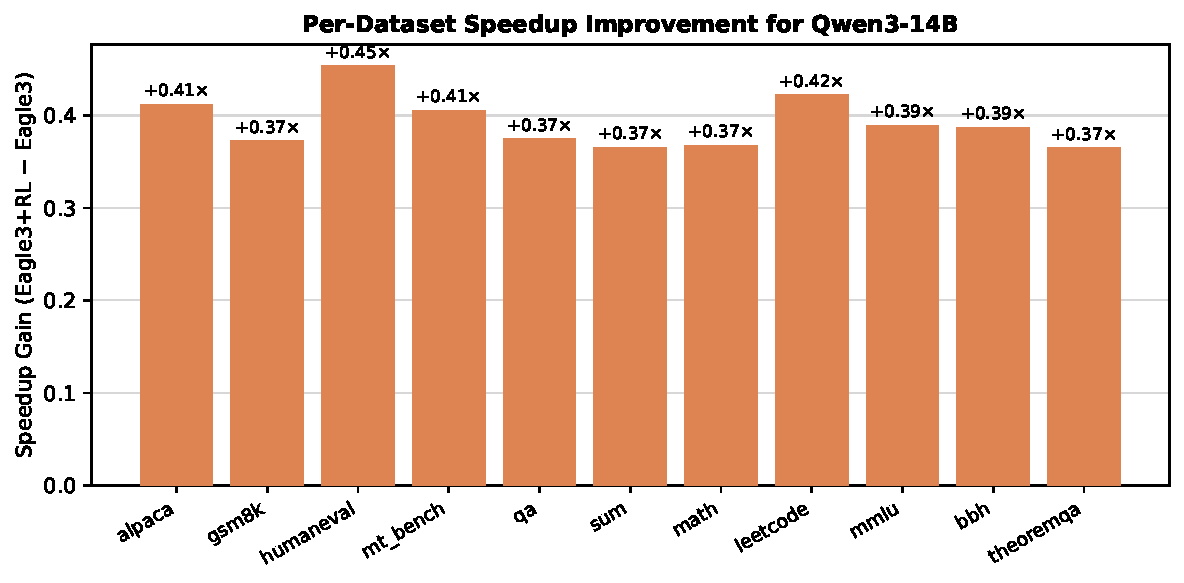
\includegraphics[width=\linewidth]{fig2_qwen_per_dataset.pdf}
  \caption{Per-dataset speedup gain (Eagle3+RL $-$ Eagle3) for Qwen3-14B. All 11 datasets show a positive improvement, confirming that the controller trained on HumanEval transfers across diverse task types.}
  \label{fig:qwen_per_dataset}
\end{figure}

\begin{table}[t]
\centering
\caption{Qwen3-32B reproduction under 8-bit quantization on H100. RL/Eagle3 reports the throughput ratio of the learned controller relative to static Eagle3.}
\label{tab:qwen32}
\small
\begin{tabular}{lccc}
\toprule
\textbf{Dataset} & \textbf{Eagle3} & \textbf{Eagle3+RL} & \textbf{RL/Eagle3} \\
\midrule
alpaca      & 2.99$\times$ & 3.19$\times$ & 1.069 \\
gsm8k       & 3.29$\times$ & 3.45$\times$ & 1.047 \\
humaneval   & 2.93$\times$ & 3.14$\times$ & 1.070 \\
mt\_bench   & 2.77$\times$ & 2.91$\times$ & 1.048 \\
qa          & 2.54$\times$ & 2.71$\times$ & 1.066 \\
sum         & 2.49$\times$ & 2.46$\times$ & 0.992 \\
math        & 3.36$\times$ & 3.60$\times$ & 1.070 \\
leetcode    & 2.95$\times$ & 3.12$\times$ & 1.058 \\
mmlu        & 3.31$\times$ & 3.47$\times$ & 1.046 \\
bbh         & 3.16$\times$ & 3.30$\times$ & 1.045 \\
theoremqa   & 3.15$\times$ & 3.41$\times$ & 1.083 \\
\midrule
\textbf{Average} & 3.00$\times$ & \textbf{3.16}$\times$ & \textbf{1.054} \\
\bottomrule
\end{tabular}
\end{table}

\paragraph{Qwen3-32B under 8-bit quantization.}
The new Qwen3-32B experiment completes the five-model reproduction. Table~\ref{tab:qwen32} shows that static Eagle3 reaches 3.00$\times$ average speedup over autoregressive decoding, while Eagle3+RL increases this to 3.16$\times$, a 5.4\% throughput gain over static Eagle3. The gain is positive on 10 of 11 datasets; summarization is the only regression, where the learned controller is slightly slower than static Eagle3 (2.46$\times$ vs. 2.49$\times$). The average acceptance length also increases from 3.72 to 3.98 tokens per speculative step. Compared with Qwen3-14B, the 32B model still benefits from adaptive control, but the margin is smaller, suggesting that the 8-bit Qwen3-32B setup is closer to a saturated static operating point.

\paragraph{Vicuna-13B-v1.3.}
Vicuna-13B achieves the highest static Eagle3 speedups in our experiments, and the average improvement from RL is correspondingly small (4.16$\times \to 4.20\times$). The depth controller almost always selects the maximum allowed depth, suggesting that for this model the learned policy is close to an ``always continue'' strategy. Moreover, the benefit of RL is uneven across datasets: it improves substantially on HumanEval and slightly on Math and LeetCode, but is neutral or slightly worse on QA, summarization, MMLU, and TheoremQA. Therefore, the Vicuna results should be interpreted as evidence that adaptive control is not uniformly beneficial once the static baseline is already very strong.

\paragraph{Acceptance length vs. speedup.}
Eagle3+RL does not always increase the average acceptance length relative to static Eagle3. This is consistent with the LTD paper's main argument: the controller is optimized for throughput rather than acceptance length itself~\cite{ltd2025}. In several cases, a similar or even slightly lower acceptance length still yields better end-to-end speedup because the controller avoids expensive draft/verification choices whose latency cost outweighs their benefit.

Figure~\ref{fig:acc_vs_speedup} makes this concrete for the initial four-model reproduction. Each point represents one model--dataset pair, with the horizontal axis showing the change in average acceptance length and the vertical axis showing the change in speedup. Many points lie in the lower-right quadrant: speedup improves despite acceptance length decreasing. This confirms that throughput-oriented optimization departs meaningfully from acceptance-length maximization.

\begin{figure}[t]
  \centering
  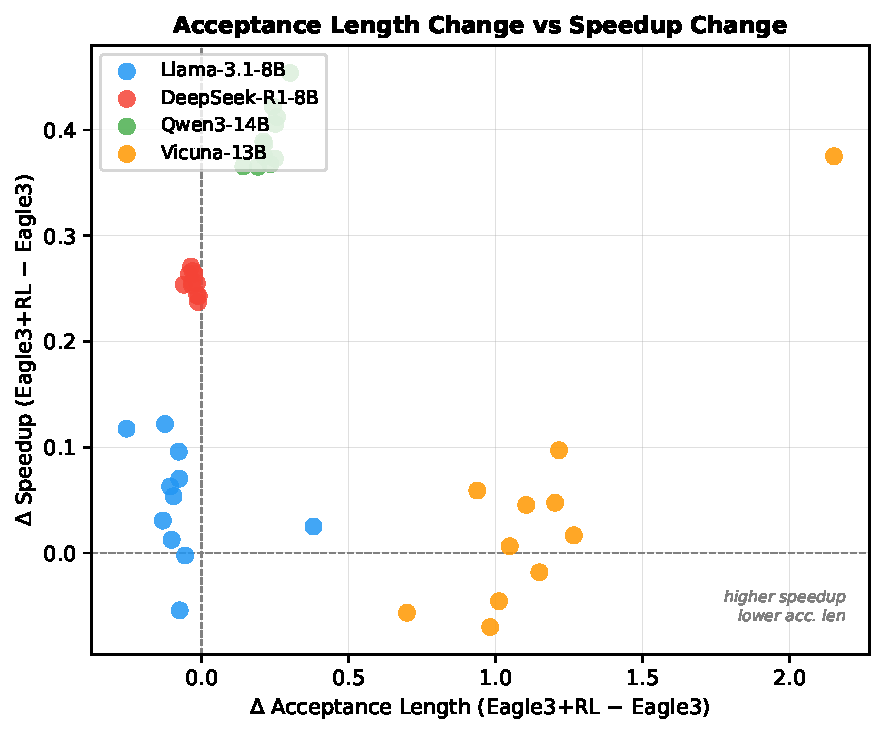
\includegraphics[width=\linewidth]{fig3_acc_vs_speedup.pdf}
  \caption{Each point is one model--dataset pair from the initial four-model reproduction. Points in the lower-right quadrant (positive $\Delta$Speedup, negative $\Delta$Acceptance Length) show that the RL controller can improve throughput even without increasing accepted tokens per step, consistent with LTD's throughput-first objective.}
  \label{fig:acc_vs_speedup}
\end{figure}

\section{Transfer and Deployment Extensions}

\paragraph{Quantization transferability.}
We next test whether a Qwen3-14B policy trained under one precision remains effective under another. Table~\ref{tab:quant_transfer} reports the average Eagle3+RL throughput divided by static Eagle3 throughput across HumanEval, Alpaca, GSM8K, and MT-Bench. Across all 36 policy--precision--dataset combinations, Eagle3+RL averages 1.056$\times$ over static Eagle3, and only two individual runs fall below 1.0$\times$. This indicates that LTD policies are mostly transferable across bf16, int4, and int8 deployment precisions.

\begin{table}[t]
\centering
\caption{Quantization transfer on Qwen3-14B. Entries are average Eagle3+RL / Eagle3 throughput ratios across four datasets.}
\label{tab:quant_transfer}
\scriptsize
\setlength{\tabcolsep}{3pt}
\begin{tabular}{lcccc}
\toprule
\textbf{Policy} & \textbf{bf16} & \textbf{int4} & \textbf{int8} & \textbf{Avg.} \\
\midrule
bf16 & 1.046 & 1.056 & 1.069 & 1.057 \\
int4 & \textbf{1.118} & 1.060 & 1.057 & \textbf{1.078} \\
int8 & 1.018 & 1.005 & \textbf{1.074} & 1.032 \\
\bottomrule
\end{tabular}
\end{table}

The strongest transfer comes from the int4-trained policy, which averages 1.078$\times$ over static Eagle3 and even improves bf16 evaluation by 11.8\%. The int8-trained policy is less robust: it is best when evaluated under int8, but it nearly matches static Eagle3 under int4 and has two dataset-level regressions. The policy action statistics explain part of this difference. The int4 policy uses a smaller verification budget (120 tokens) and shallower depth, while the int8 policy uses a larger budget (210 tokens) and deeper trees. The more aggressive int8 policy appears more sensitive to changes in precision-specific latency and acceptance behavior.

\begin{figure*}[t]
  \centering
  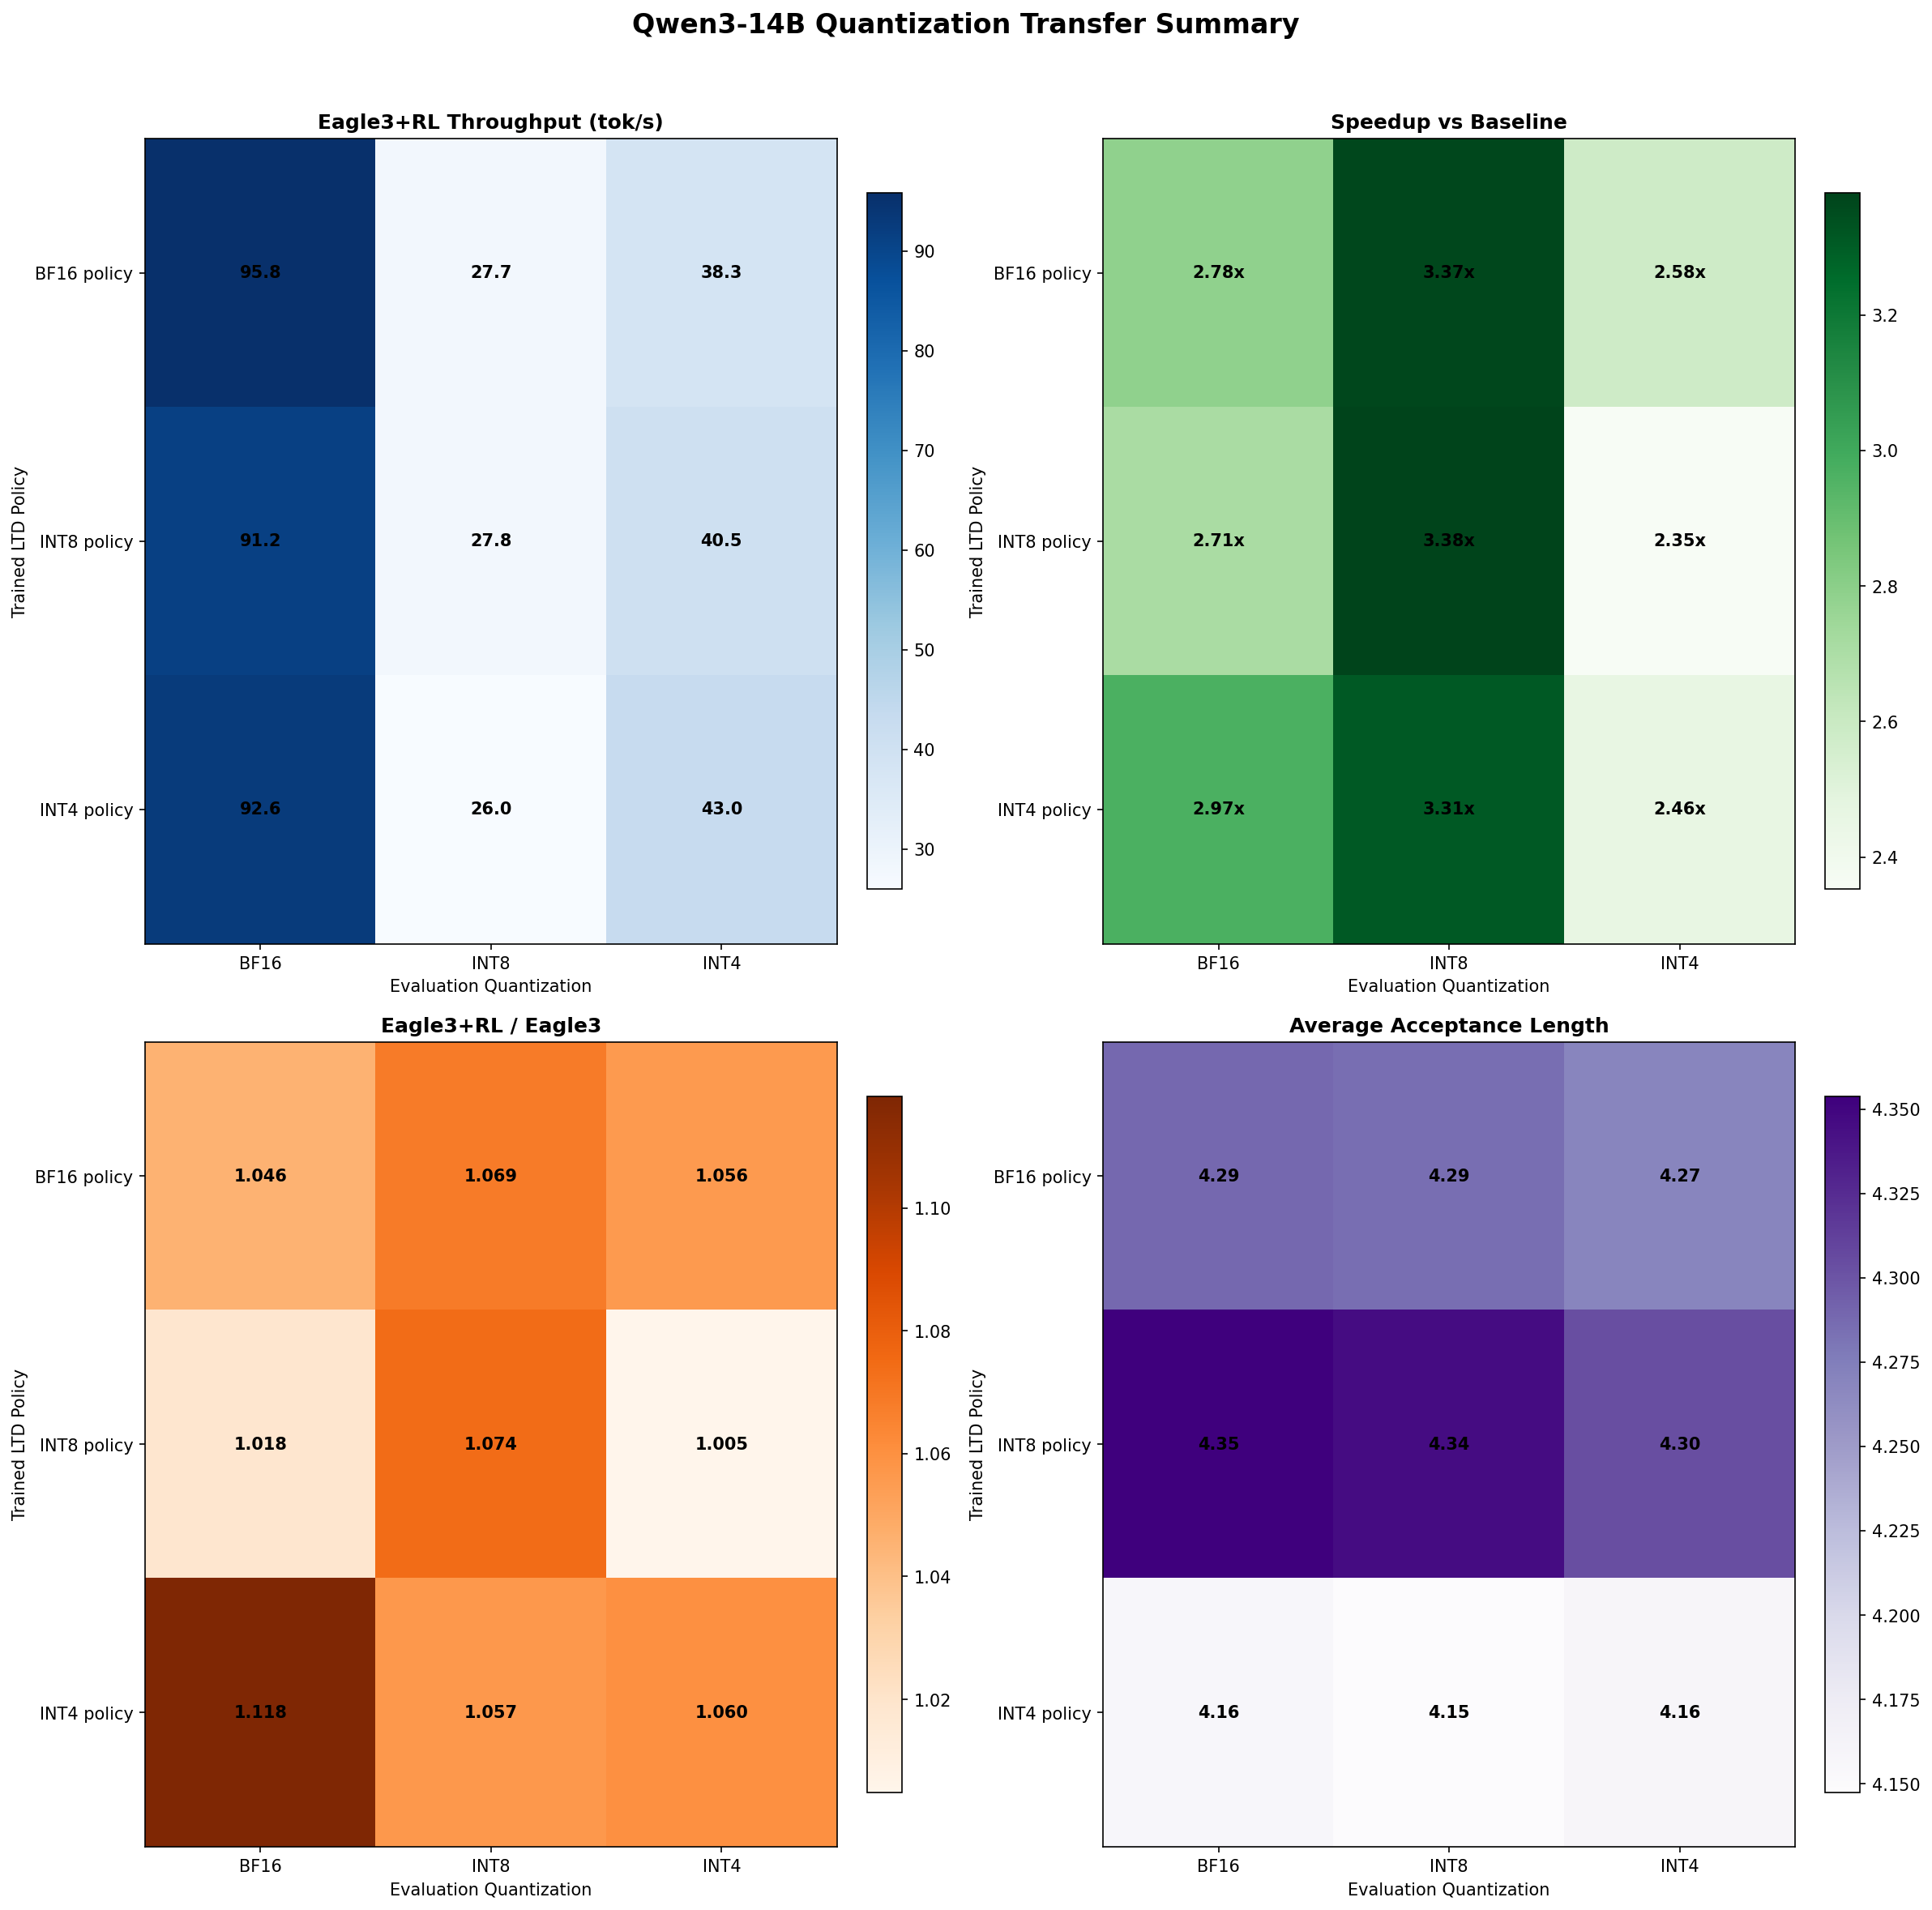
\includegraphics[width=0.72\textwidth]{quant_transfer_summary_charts.png}
  \caption{Quantization-transfer summary for Qwen3-14B. The learned policies generally remain faster than static Eagle3 across deployment precisions, but the int8-trained policy is the least robust when moved to other precisions.}
  \label{fig:quant_transfer}
\end{figure*}

\paragraph{Hardware transferability.}
Hardware transfer is much weaker. Table~\ref{tab:hardware_transfer} evaluates bf16 Qwen3-14B policies trained on A5090 or H100 when deployed on an RTX A6000. Both transferred policies remain faster than the autoregressive baseline, but both are substantially slower than static Eagle3 on the target GPU. The A5090-trained policy averages only 0.693$\times$ of static Eagle3 throughput, while the H100-trained policy reaches 0.739$\times$.

\begin{table}[t]
\centering
\caption{Hardware transfer on Qwen3-14B bf16. Policies trained on A5090 or H100 are evaluated on RTX A6000.}
\label{tab:hardware_transfer}
\scriptsize
\setlength{\tabcolsep}{2.5pt}
\begin{tabular}{lccccc}
\toprule
\textbf{Train} & \textbf{E3 sp.} & \textbf{RL sp.} & \textbf{RL/E3} & \textbf{Size} & \textbf{Depth} \\
\midrule
A5090 & 2.55$\times$ & 1.76$\times$ & 0.693 & 220 & 4.09 \\
H100  & 2.55$\times$ & 1.89$\times$ & 0.739 & 190 & 5.21 \\
\bottomrule
\end{tabular}
\end{table}

This result is the clearest evidence that LTD's throughput reward is hardware-specific. The learned policy internalizes the latency trade-off of the training GPU: how expensive extra draft expansion is, how well larger verification batches are amortized, and where memory bandwidth becomes limiting. When moved to an RTX A6000, those trade-offs change enough that the learned actions become worse than the static Eagle3 heuristic.

\begin{figure*}[t]
  \centering
  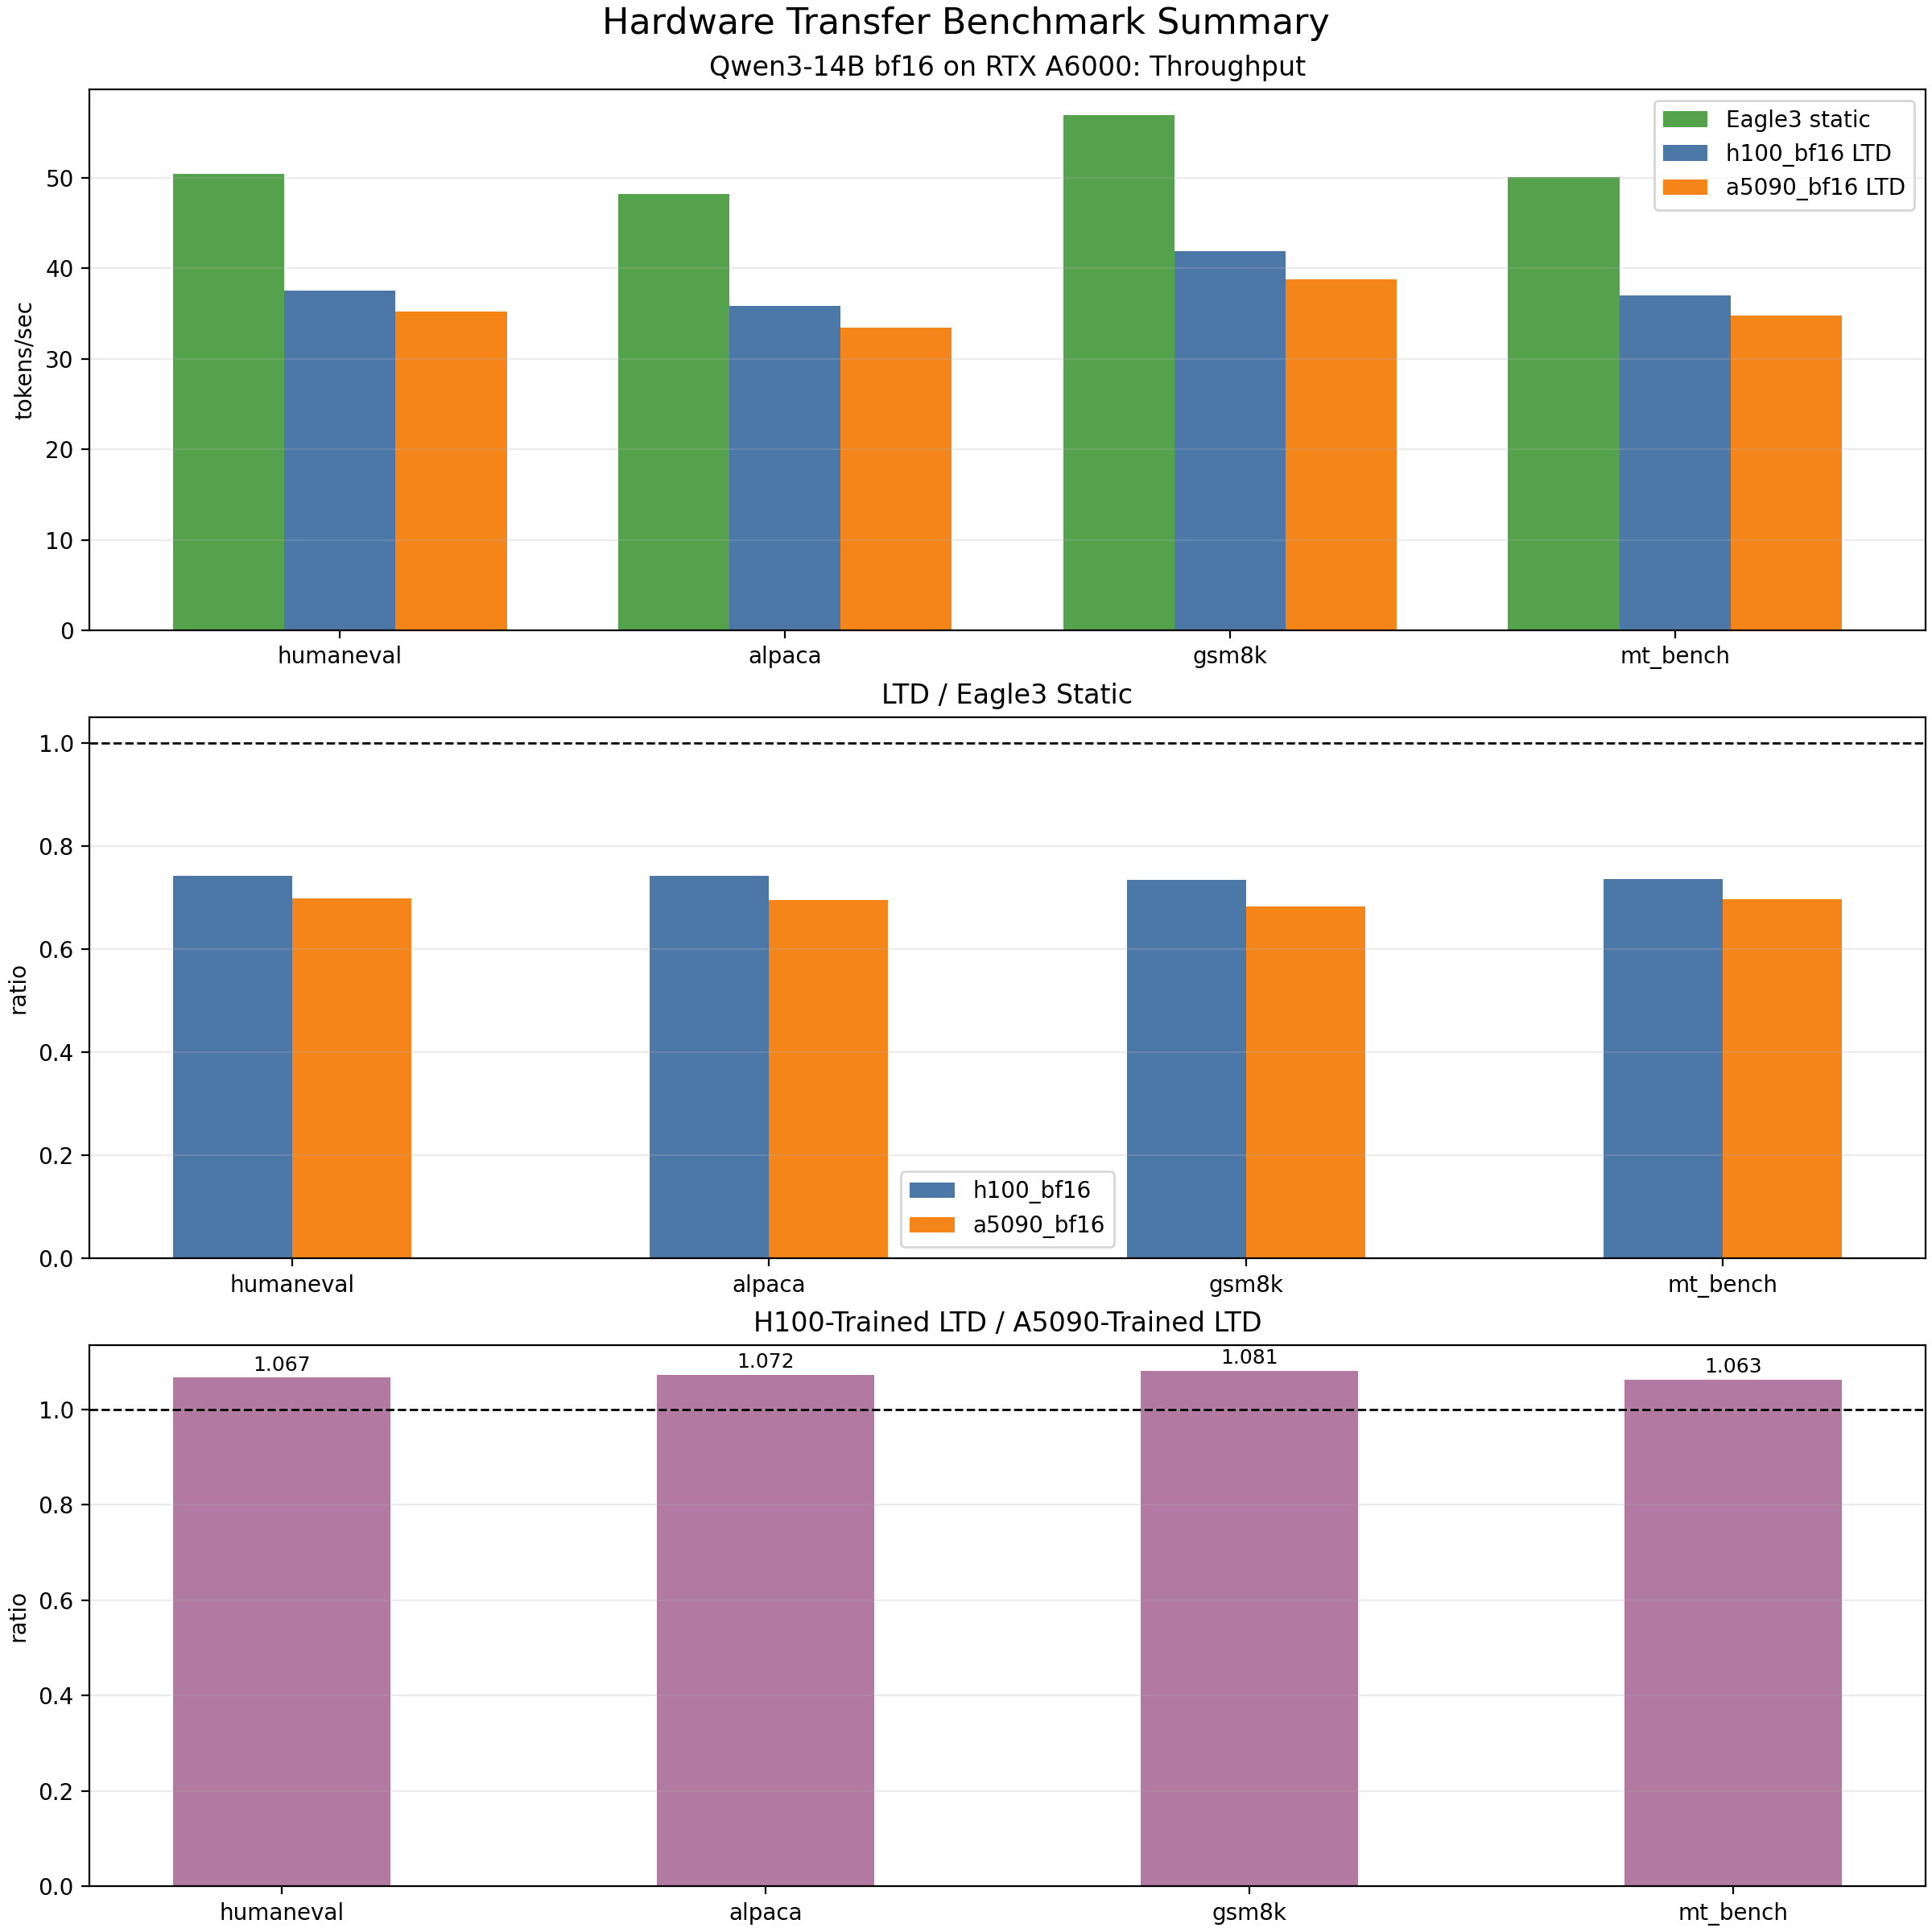
\includegraphics[width=0.72\textwidth]{hardware_transfer_summary_charts.png}
  \caption{Hardware-transfer summary for Qwen3-14B bf16. Transferred policies still beat autoregressive decoding, but they fail to beat static Eagle3 on RTX A6000.}
  \label{fig:hardware_transfer}
\end{figure*}

\paragraph{Naive two-GPU model parallelism.}
Finally, we evaluate whether LTD remains effective when Qwen3-32B is split across two GPUs using naive layer sharding. Table~\ref{tab:twogpu} compares the single-GPU and two-GPU Qwen3-32B 8-bit runs. The relative speedups are almost unchanged: Eagle3+RL is 1.054$\times$ over static Eagle3 on one GPU and 1.053$\times$ under the two-GPU device map. However, absolute throughput drops by about 8\% for all methods under two-GPU sharding.

\begin{table}[t]
\centering
\caption{Qwen3-32B 8-bit under single-GPU and naive two-GPU model parallelism. Throughput is averaged across all 11 datasets.}
\label{tab:twogpu}
\scriptsize
\setlength{\tabcolsep}{2.5pt}
\begin{tabular}{lccccc}
\toprule
\textbf{Setting} & \textbf{Base tp} & \textbf{E3 tp} & \textbf{RL tp} & \textbf{RL sp.} & \textbf{RL/E3} \\
\midrule
1 GPU & 5.60 & 16.75 & 17.67 & 3.16$\times$ & 1.054 \\
2 GPUs & 5.11 & 15.36 & 16.19 & 3.17$\times$ & 1.053 \\
\bottomrule
\end{tabular}
\end{table}

Thus, naive model parallelism does not provide a throughput win in this setting; it mainly makes the model easier to place in memory. Still, the learned LTD controller remains effective under sharding because the relative speculative-decoding trade-off is preserved. A more promising direction would be true pipeline or tensor parallel speculative decoding, where multiple GPUs reduce verification latency rather than only partitioning model layers.

\section{Discussion and Future Work}

\paragraph{Progress summary.}
We have successfully reproduced the core LTD pipeline on five target models and verified its main qualitative conclusion: reinforcement-learning-based adaptive control improves throughput over static EAGLE-3 in most same-hardware, same-precision settings. Relative to the original paper, our extensions now include broader dataset coverage, Qwen3-32B under 8-bit quantization, quantization-transfer sweeps, hardware-transfer sweeps, and a naive two-GPU deployment study.

\paragraph{When does adaptive control help most?}
Our results suggest that adaptive control helps most when the static Eagle3 operating point is far from optimal and the deployment condition matches training. This is especially clear for DeepSeek-R1-Distill-Llama-8B and Qwen3-14B, where the average gains are substantial. By contrast, when static Eagle3 already performs very well, as in Llama-3.1-8B and Vicuna-13B, the learned controller has much less room to improve and may only help on specific task categories. Qwen3-32B falls between these cases: it benefits consistently under 8-bit quantization, but the average gain is only 5.4\%.

Figure~\ref{fig:saturation} plots each model--dataset pair from the initial reproduction with static Eagle3 speedup on the horizontal axis and the RL gain ($\text{Eagle3+RL} - \text{Eagle3}$) on the vertical axis. The negative trend line confirms the saturation hypothesis quantitatively: as the static baseline approaches its ceiling, the marginal benefit of adaptive control diminishes.

\begin{figure}[t]
  \centering
  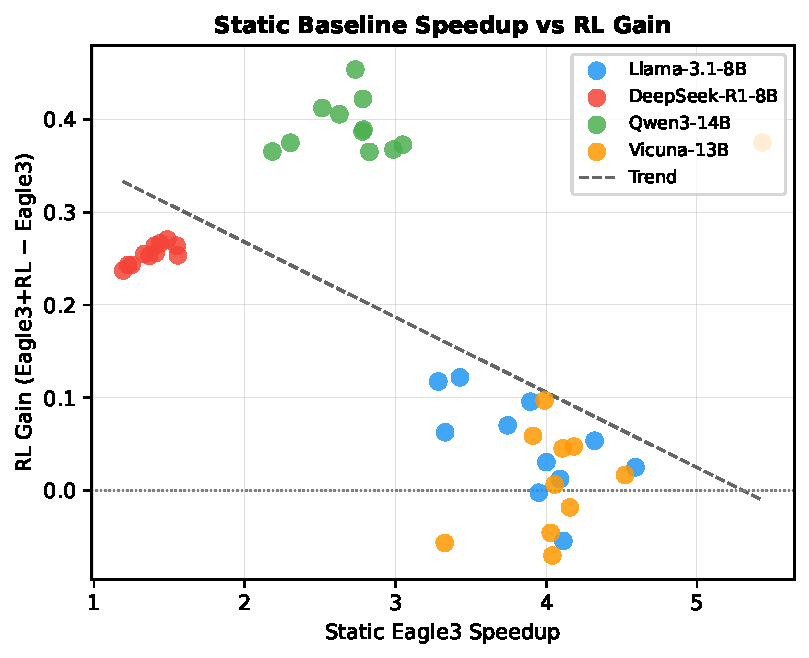
\includegraphics[width=\linewidth]{fig4_saturation.pdf}
  \caption{Static Eagle3 speedup versus RL gain for every model--dataset pair in the initial reproduction. The dashed trend line shows a negative correlation: stronger static baselines leave less room for the RL controller to improve, validating the saturation hypothesis.}
  \label{fig:saturation}
\end{figure}

\paragraph{Limitations.}
The current experiments only cover greedy decoding. The original LTD paper also studies temperature-1 sampling and reports that adaptive control remains effective in that setting~\cite{ltd2025}. In addition, our policies are trained only on HumanEval, so the current results do not isolate how much of the observed transfer comes from the policy design itself versus the specific training distribution. The transfer experiments are also smaller than the main reproduction: quantization and hardware transfer use four datasets, and hardware transfer only tests deployment on one target GPU. Finally, the two-GPU experiment uses naive layer sharding, not communication-aware pipeline or tensor parallelism.

\paragraph{Next steps.}
Useful next steps are:
\begin{denseitemize}
  \item evaluate under sampling (temperature $> 0$) and compare against the paper's reported trends;
  \item study alternative reward functions, such as acceptance-length-only and latency-aware objectives;
  \item analyze controller decisions more directly through distributions of selected size and depth actions;
  \item investigate whether hardware-conditioned features or lightweight target-GPU fine-tuning can improve hardware transfer;
  \item explore true distributed speculative decoding, where drafting and verification are pipelined or tensor-parallelized across GPUs to measure whether overlap can outweigh communication overhead.
\end{denseitemize}

\bibliographystyle{unsrt}
\bibliography{rlps}

\appendix

\section{Full Per-Dataset Statistics}
\label{app:full_stats}

Table~\ref{tab:full_stats} reports per-dataset acceptance length, draft size, depth stop, and speedup for the initial four-model reproduction. Several findings from the main text are directly visible here: (1)~Vicuna-13B consistently reaches DepthStop~$= 12.00$, confirming the depth controller defaults to ``always continue''; (2)~DeepSeek-R1-8B has acceptance lengths below 2.5 across all datasets, explaining why static Eagle3 yields only modest speedups; (3)~Qwen3-14B gains are uniformly positive and spread across task types, supporting cross-task generalisation.

\begin{table*}[t]
\centering
\caption{Per-model, per-dataset statistics for Eagle3 and Eagle3+RL.
Acc.~Len = average accepted tokens per speculative step;
SizeTok = average number of draft tokens selected by the size policy;
DepthStop = average tree depth at which the depth policy halts;
Speedup = throughput ratio relative to the autoregressive baseline.}
\label{tab:full_stats}
\scriptsize
\setlength{\tabcolsep}{4pt}
\begin{tabular}{lcccccc}
\toprule
 & \multicolumn{2}{c}{\textbf{Eagle3}} & \multicolumn{4}{c}{\textbf{Eagle3+RL}} \\
\cmidrule(lr){2-3}\cmidrule(lr){4-7}
\textbf{Dataset} & \textbf{Acc.~Len} & \textbf{Speedup}
                 & \textbf{Acc.~Len} & \textbf{SizeTok} & \textbf{DepthStop} & \textbf{Speedup} \\
\midrule
\multicolumn{7}{l}{\textit{Llama-3.1-8B-Instruct}} \\
Alpaca      & 6.96 & 4.32$\times$ & 6.86 & 49.4 & 7.22 & 4.37$\times$ \\
GSM8K       & 6.47 & 4.09$\times$ & 6.37 & 50.0 & 7.10 & 4.10$\times$ \\
HumanEval   & 7.23 & 4.59$\times$ & 7.61 & 50.0 & 8.58 & 4.62$\times$ \\
MT-Bench    & 6.29 & 4.00$\times$ & 6.16 & 50.0 & 6.74 & 4.03$\times$ \\
QA          & 5.22 & 3.28$\times$ & 4.97 & 50.0 & 5.56 & 3.40$\times$ \\
Sum         & 5.40 & 3.43$\times$ & 5.28 & 50.0 & 6.02 & 3.55$\times$ \\
Math        & 6.22 & 3.95$\times$ & 6.16 & 50.0 & 7.26 & 3.95$\times$ \\
LeetCode    & 6.44 & 4.11$\times$ & 6.37 & 50.0 & 7.52 & 4.06$\times$ \\
MMLU        & 5.83 & 3.74$\times$ & 5.75 & 50.0 & 6.65 & 3.81$\times$ \\
BBH         & 6.07 & 3.90$\times$ & 5.99 & 50.0 & 6.50 & 3.99$\times$ \\
TheoremQA   & 5.17 & 3.33$\times$ & 5.06 & 50.0 & 6.49 & 3.39$\times$ \\
\midrule
\multicolumn{7}{l}{\textit{DeepSeek-R1-Distill-Llama-8B}} \\
Alpaca      & 1.89 & 1.23$\times$ & 1.88 & 60.0 & 3.04 & 1.47$\times$ \\
GSM8K       & 2.40 & 1.56$\times$ & 2.34 & 60.0 & 3.15 & 1.81$\times$ \\
HumanEval   & 2.29 & 1.49$\times$ & 2.26 & 60.0 & 3.07 & 1.76$\times$ \\
MT-Bench    & 2.11 & 1.37$\times$ & 2.07 & 60.0 & 3.08 & 1.62$\times$ \\
QA          & 1.84 & 1.19$\times$ & 1.82 & 60.0 & 3.03 & 1.43$\times$ \\
Sum         & 1.93 & 1.25$\times$ & 1.92 & 60.0 & 3.02 & 1.49$\times$ \\
Math        & 2.39 & 1.55$\times$ & 2.35 & 60.0 & 3.17 & 1.81$\times$ \\
LeetCode    & 2.16 & 1.40$\times$ & 2.13 & 60.0 & 3.06 & 1.67$\times$ \\
MMLU        & 2.06 & 1.33$\times$ & 2.04 & 60.0 & 3.08 & 1.59$\times$ \\
BBH         & 2.22 & 1.44$\times$ & 2.19 & 60.0 & 3.09 & 1.70$\times$ \\
TheoremQA   & 2.17 & 1.41$\times$ & 2.14 & 60.0 & 3.10 & 1.67$\times$ \\
\midrule
\multicolumn{7}{l}{\textit{Qwen3-14B}} \\
Alpaca      & 3.59 & 2.51$\times$ & 3.85 & 220.0 & 3.89 & 2.93$\times$ \\
GSM8K       & 4.36 & 3.05$\times$ & 4.61 & 220.0 & 4.55 & 3.42$\times$ \\
HumanEval   & 3.90 & 2.73$\times$ & 4.21 & 220.0 & 3.98 & 3.19$\times$ \\
MT-Bench    & 3.75 & 2.63$\times$ & 4.00 & 220.0 & 3.91 & 3.03$\times$ \\
QA          & 3.28 & 2.30$\times$ & 3.49 & 220.0 & 3.75 & 2.68$\times$ \\
Sum         & 3.14 & 2.18$\times$ & 3.28 & 220.0 & 3.16 & 2.55$\times$ \\
Math        & 4.27 & 2.99$\times$ & 4.50 & 220.0 & 4.43 & 3.35$\times$ \\
LeetCode    & 3.97 & 2.78$\times$ & 4.22 & 220.0 & 3.93 & 3.21$\times$ \\
MMLU        & 3.98 & 2.79$\times$ & 4.19 & 220.0 & 4.03 & 3.18$\times$ \\
BBH         & 3.97 & 2.78$\times$ & 4.18 & 220.0 & 4.03 & 3.17$\times$ \\
TheoremQA   & 4.04 & 2.83$\times$ & 4.24 & 220.0 & 4.16 & 3.19$\times$ \\
\midrule
\multicolumn{7}{l}{\textit{Vicuna-13B-v1.3}} \\
Alpaca      & 6.23 & 3.91$\times$ & 7.17  & 200.0 & 12.00 & 3.97$\times$ \\
GSM8K       & 6.25 & 4.06$\times$ & 7.30  & 200.0 & 12.00 & 4.06$\times$ \\
HumanEval   & 8.35 & 5.43$\times$ & 10.50 & 200.0 & 12.00 & 5.81$\times$ \\
MT-Bench    & 6.42 & 4.11$\times$ & 7.53  & 197.5 & 11.85 & 4.15$\times$ \\
QA          & 5.18 & 3.33$\times$ & 5.88  & 200.0 & 12.00 & 3.27$\times$ \\
Sum         & 6.66 & 4.16$\times$ & 7.81  & 200.0 & 12.00 & 4.14$\times$ \\
Math        & 6.16 & 3.99$\times$ & 7.38  & 200.0 & 12.00 & 4.09$\times$ \\
LeetCode    & 6.89 & 4.52$\times$ & 8.15  & 200.0 & 12.00 & 4.54$\times$ \\
MMLU        & 6.14 & 4.03$\times$ & 7.15  & 200.0 & 12.00 & 3.98$\times$ \\
BBH         & 6.41 & 4.18$\times$ & 7.61  & 200.0 & 12.00 & 4.23$\times$ \\
TheoremQA   & 6.15 & 4.04$\times$ & 7.13  & 200.0 & 12.00 & 3.97$\times$ \\
\bottomrule
\end{tabular}
\end{table*}

\end{document}
